\documentclass[tikz]{standalone}

\usepackage{amsmath}
\usetikzlibrary{shapes,arrows,shadows,calc, angles}
\usetikzlibrary{arrows,shapes}
\usetikzlibrary{positioning}
\usetikzlibrary{patterns.meta}

\usetikzlibrary{decorations, decorations.pathreplacing}

\definecolor{fg}{rgb}{0,0,0}
\definecolor{bg}{rgb}{1,1,1}

\tikzstyle{box}=[draw, rounded corners, thick,
anchor=center,text centered,text=fg, font=\bfseries] % text width=33mm,

\tikzstyle{myarrow}=[->, >=stealth, thick, rounded corners=4mm]
\tikzstyle{mythinarrow}=[myarrow, line width=0.25mm]

\begin{document}

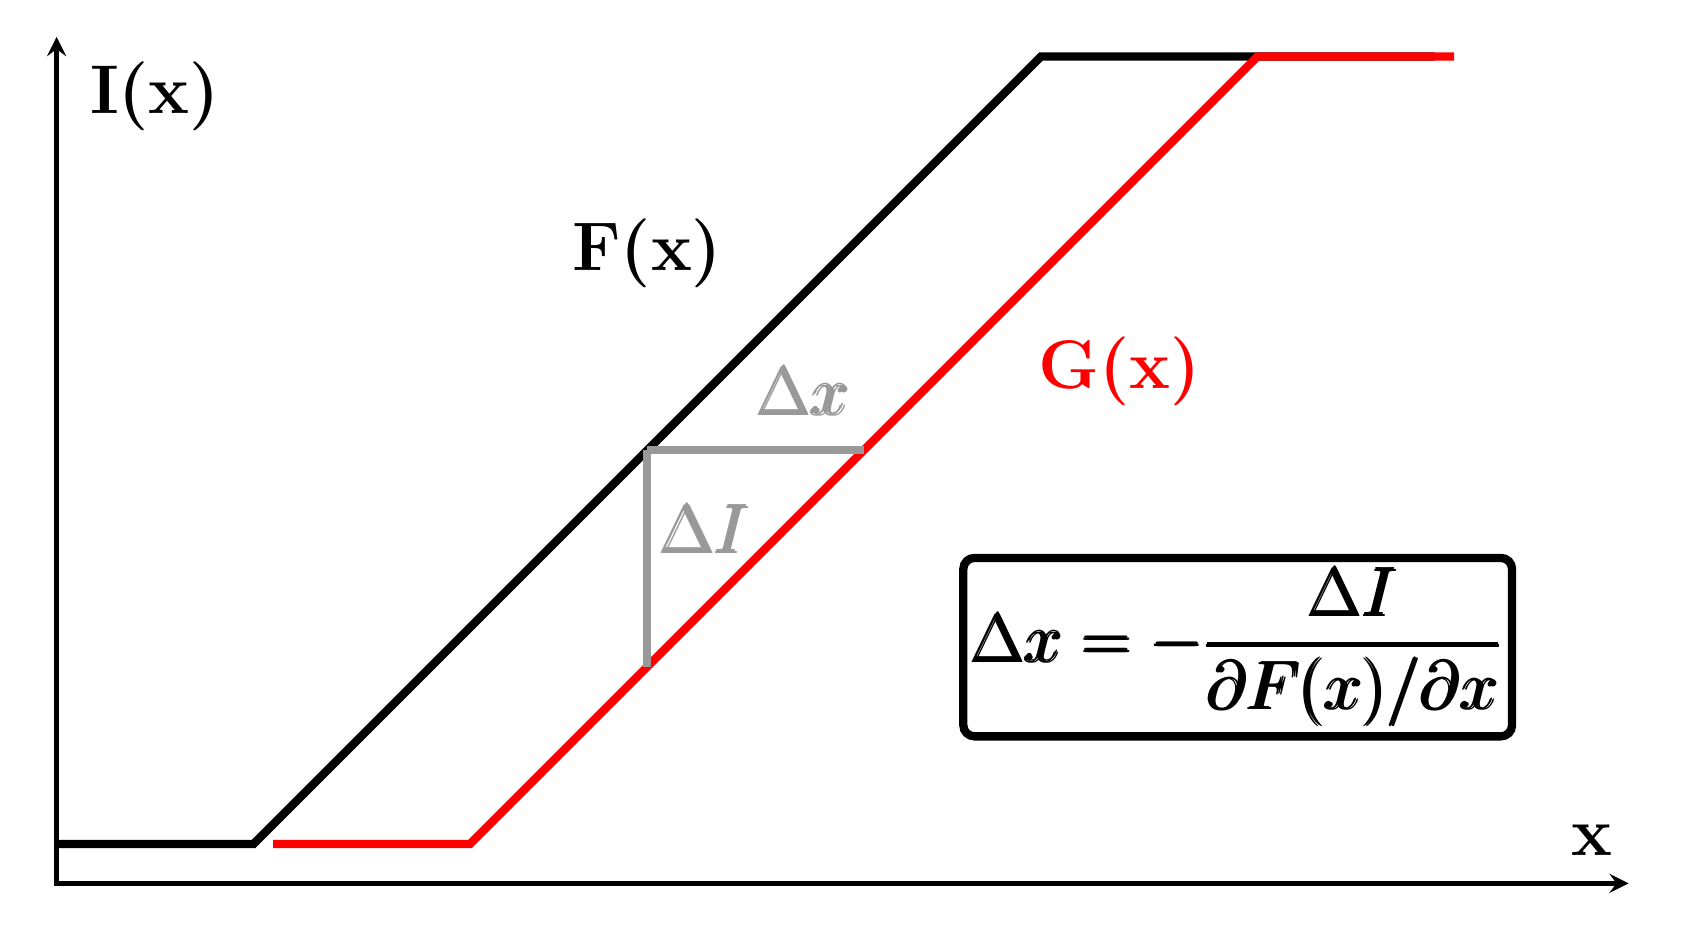
\begin{tikzpicture}[scale=5, font=\bfseries\fontsize{25}{14}\selectfont, line width=3]
    %\draw[help lines] grid (5, 3) ;
    \node at (-0.05, -0.15) {} ;
    \node at (4.05, 2.05) {} ;
    % \draw[line width=1] (-1, 0) -- (1, 0) -- (0,0) -- (0, 2) -- (0, -2) ;
    \draw[myarrow, line width=2] (-0.007, -0.1) -- ++ (4, 0) ;
    \draw[myarrow, line width=2] (0, -0.1) -- ++ (0, 2.15) ;
    \node at (3.9, 0.01) {x} ;
    \node at (0.25, 1.9) {I(x)} ;
    \draw (0, 0) -- ++ (0.5, 0) -- ++(2, 2) -- ++(1, 0) ;
    \draw[red] (0.55, 0) -- ++ (0.5, 0) -- ++(2, 2) -- ++(0.5, 0) ;
    \node (fx) at (1.5,1.5) {F(x)} ;
    \node[color=red] (gx) at (2.7,1.2) {G(x)} ;
    \draw[color=black!40] (1.5,1) -- ++(0.55,0) ;
    \node[color=black!40, text centered] at (1.9, 1.15) {$\pmb{\Delta x}$} ;
    \draw[color=black!40] (1.5,1) -- ++(0,0-0.55) ;
    \node[color=black!40, text centered] at (1.65, 0.8) {$\pmb{\Delta I}$} ;
    \node[draw, rounded corners, text centered]
        at (3, 0.5) {$\pmb{\Delta x = -\dfrac{\Delta I}{\partial F(x)/\partial x}}$ } ;
\end{tikzpicture}

\end{document}